\section{Planning and Learning with Tabular Methods}
RL methods can be described as either \textit{model-based} or \textit{model-free}. Model-based methods rely on \textit{planning} as their primary component, while model-free methods rely on \textit{learning}. Despite their differences, both still use value functions and both make backups to state values based on future returns or estimates. This chapter will provide a unifying framework for model-free and model-based RL methods.

\subsection{Models and Planning}
\begin{itemize}
	\item Models are anything the agent can use to predict the outcome of its actions.
	\item Models can be either \textit{distribution models} or \textit{sample models}. The former is a probability distribution over all possible next states whereas the latter produces one of the possible next states sampled from the probability distribution.
	\item Distribution models are stronger than sample models because they can always be used to create samples, but sample models are easier to create in practice.
	\item Models are used to \textit{simulate} the environment thus producing \textit{simulated experience}. Distribution models could produce every possible episode, weighted by their probability of occurring, whereas sample models can only produce one episode.
	\item The word \textit{planning} refers to any computational process that takes a model as input and produces or improves a policy for interacting with the modelled environment.
	\item The common structure of updating our policy by utilising our model is given in Figure \ref{fig: updating policy using model}.
	\item We can use models in place of the real environment to perform model-free learning safely i.e. using simulated experience rather than real experience.
\end{itemize}

\begin{figure} [h!]
	\centering
	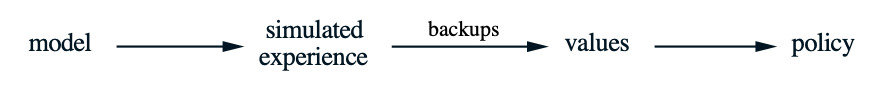
\includegraphics[width=\textwidth]{/chapter8_1}
	\caption{The framework for updating our policy using our model of the environment}
	\label{fig: updating policy using model}
\end{figure}

\subsection{Dyna: Integrated Planning, Acting, and Learning}
Instead of planning all possible future states permutation, we may want to plan over a small number of future timesteps. When we do this we will likely want to update both our policy and model \textit{online}. The canonical algorithm for doing so is \textbf{Dyna-Q}. 
\begin{itemize}
\item Planning agents can use the experience they collect to do one of two things: 1) improve the model (also called \textit{model-learning}) and 2) improve the value function and policy (also called \textit{direct reinforcement learning (direct RL)}). These options are summarised in  \ref{fig: direct rl and model-learning}. Sometimes model-learning is called \textit{indirect RL} because improving our model, improves our policy by proxy.
\item Dyna-Q agents conduct direct RL, planning, model-learning and acting simultaneously. Planning and direct learning tend to use exactly the same machinery as each other e.g. $n$-step sarsa, and thus are closely linked. Figure \ref{fig: dyna} shows the generalised Dyna architecture.
\item Planning (in Dyna Q) is the process of running our Q updates (from Q-learning) using our model. We select random states and actions previously taken, find the reward and next state using our model and make the Q update. We do this $n$ times for each timestep taken in the real environment, where $n$ is a hyper parameter. For each unit of real experience collected, we are updated our value function $n$ simultaneously.
\end{itemize}

\begin{figure}
	\centering
	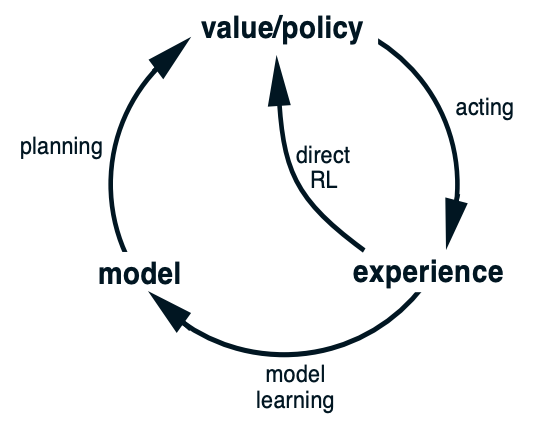
\includegraphics[width=0.5\textwidth]{/chapter8_2}
	\caption{Direct RL and model-learning, either achieved using data collected from experience}
	\label{fig: direct rl and model-learning}
\end{figure}

\begin{figure}
	\centering
	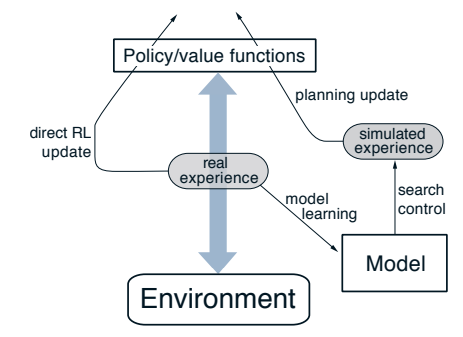
\includegraphics[width=0.5\textwidth]{/chapter8_3}
	\caption{Generalised Dyna architecture}
	\label{fig: dyna}
\end{figure}

\subsection{When the Model is Wrong}
Often our model will be wrong. This can happen initially because the environment is stochastic and we haven't collected enough samples to evaluate this stochasticty accurately. Otherwise, it can happen because we've used function approximation (e.g. neural networks) to predict the model, which generally arrive with non-zero error. When the model is incorrect the planning process is likely to compute a suboptimal policy. Often the suboptimal policy quickly leads to the discovery and correction of modelling error, as when the agent takes actions prescribed by the planned policy in the real environment, it quickly finds the expected rewards are incorrect or do not exist. 

Issues arise when the environment changes to become \textit{better} or more favourable at some stage during learning. In these cases the optimal policy/route to goal remains unchanged, but there is an even better policy available that the agent may never access because it has no reason to doubt its previously learned optimal policy. To address this, another algorithm is proposed called Dyna-Q+. Here, the agent keeps track of the number of timesteps elapsed $\tau$ since a state-action pair had been selected, and, if sufficient time has elapsed, it is presumed that the dynamics of the environment from that state have changed. The modelled rewards for each state-action pair now take the form $r + k\sqrt{\tau}$ for some small $k$.

